\documentclass{article}
\usepackage[UTF8]{ctex}
\usepackage{geometry}
\usepackage{natbib}
\geometry{left=3.18cm,right=3.18cm,top=2.54cm,bottom=2.54cm}
\usepackage{graphicx}
\pagestyle{plain}	
\usepackage{setspace}
\usepackage{caption2}
\usepackage{datetime} %日期
\renewcommand{\today}{\number\year 年 \number\month 月 \number\day 日}
\renewcommand{\captionlabelfont}{\small}
\renewcommand{\captionfont}{\small}
\begin{document}

\begin{figure}
    \centering
    
\includegraphics[width=8cm]{upc.png}

    \label{figupc}
\end{figure}

	\begin{center}
		\quad \\
		\quad \\
		\heiti \fontsize{45}{17} \quad \quad \quad 
		\vskip 1.5cm
		\heiti \zihao{2} 《计算科学导论》课程总结报告
	\end{center}
	\vskip 2.0cm
		
	\begin{quotation}
% 	\begin{center}
		\doublespacing
		
        \zihao{4}\par\setlength\parindent{7em}
		\quad 

		学生姓名:\underline{\qquad  李福静 \qquad \qquad}

		学\hspace{0.61cm} 号:\underline{\qquad 1907010203\qquad}
		
		专业班级:\underline{\qquad 计科1902 \qquad  }
		
        学\hspace{0.61cm} 院:\underline{计算机科学与技术学院}
% 	\end{center}
		\vskip 2cm
		\centering
		\begin{table}[h]
            \centering 
            \zihao{4}
            \begin{tabular}{|c|c|c|c|c|c|c|}
            % 这里的rl 与表格对应可以看到,姓名是r,右对齐的;学号是l,左对齐的;若想居中,使用c关键字。
                \hline
                课程认识 & 问题思 考 & 格式规范  & IT工具  & Latex附加  & 总分 & 评阅教师 \\
                30\% & 30\% & 20\% & 20\% & 10\% &  &  \\
                \hline
                 & & & & & &\\
                & & & & & &\\
                \hline
            \end{tabular}
        \end{table}
		\vskip 2cm
		\today
	\end{quotation}

\thispagestyle{empty}
\newpage
\setcounter{page}{1}
% 在这之前是封面,在这之后是正文
\section{引言}
导论的目的在于从科学哲学的角度用高级科普的形式为初学者提供一个了解和学习计算机科学与技术领域的专门的,具体的,系统的专业技术知识。导论并不系统地阐述科学哲学与学科方法论的内容,而是将科学哲学的观点与学科方法论中大量成熟的内容融入到各章节之中,自始至终贯穿在各个章节的字里行间中。导论中很少涉及具体的,系统的专业知识特别是操作使用计算机的技术知识,因为导论仅是为我们以后学习基础课程和后续计算机科学与技术的一个导引。其中没有解释的一些名词和术语,以后会在一些具体的分支学科课程中学到,其中的许多观点和思想方法,对整个大学生涯是大有裨益的。
\section{对计算科学导论这门课程的认识、体会}
通过《计算科学导论》的学习。我或深或浅地了解了计算模型与二进制,存储程序式计算机的基本结构与工作原理,数字逻辑与集成电路,机器指令与汇编语言,算法、过程与程序,高级语言与程序设计,系统软件与应用软件,计算机组织与体系结构,并行计算机、通道与并行计算,计算机网络与通信,计算机图形学与图像处理,逻辑与人工智能,计算机科学与技术一级学科等领域内的一些重要的基本概念。该书还围绕计算机科学与技术学科的定义、特点、基本问题、发展主线、主流方向、学科方法论、历史渊源、发展变化等内容进行了系统且深入浅出的论述,以科学办学思想和内涵发展优先的理念为基础,全面阐述了如何使学生正确地认识和学好计算机科学与技术学科。一切科学理论只有在赋予哲学解释之后才能获得升华。站在科学哲学的高度,采用高级科普的形式去认知和引导学习计算机科学与技术学科是《计算科学导论》的鲜明特色之一。值得注意的是,该书并没有专门系统地阐述科学哲学和学科方法论的内容,而是将科学哲学的观点和学科方法论中大量成熟的内容融入到各章节之中,自始至终贯彻在各个章节的字里行间。\par
孙老师常说,把教材当成一本科普书,常翻常看。《计算科学导论》是一本很有意思的书,尽管有一部分,甚至很大一部分我虽读了几遍还是朦朦胧胧,但这些理论知识正逐渐渗入我的思想中,进一步的理解和提高需要时间和更多的知识储备。我想分享的两部分内容是算法、过程与程序和计算机网络与通信。
\par

\subsection{算法、过程与程序}
在书中大致了解了相关概念以后,我对算法程序产生了兴趣,又因为是计算机专业,平时也在接触一些简单的算法,所以我阅读了《Relief算法最佳数学降维过程的程序实现》[1],了解了Relief算法,开拓了我的视野,也激起了我对算法的研究热情,我后续也在尝试着在算法的领域不断深入,并计划坚持对算法、程序的探索,希望有更多的收获!
\subsection{计算机网络与通信}
伴随着科技日新月异的发展,计算机网络与通信逐渐走入人们视线。在对计算机网络与通信的发展历史与原理有了简单的了解之后,我对网络安全方面有所深入。阅读了《计算机网络技术在通信工程项目管理中的应用初探》[2],使我对计算机网络技术应用到生活的多样化有了新的认识,发散了我的思维,同时,我也对安全性产生了疑惑。于是又查阅了《计算机网络通信安全中数据加密技术的应用》[3],了解了数据加密技术在生活中的应用,应用与保护齐头并进,让科学走入生活。这让我对计算机行业未来的发展充满了期待。在学习期间还看了一篇《Analog Neural Networks with Deep-submicron Nonlinear Synapses》[4]的论文,它为我科普了计算机网络的新知识,使我对计算机专业的热爱更加深厚! 

\section{进一步的思考}
在学习了更多的计算机专业有关的知识后,我对我们组《云桌面》在演讲过程中存在的问题进行了更深入的思考,并查阅了相关资料,现将其完善。\par

\begin{itemize}
    \item 	VDI和VOI协同工作的云桌面管理模式。\par
    在演讲过程中,我们介绍了VDI与VOI的优缺点,却并未提及解决方案。《云桌面VDI和VOI工作模式的协同研究》[5]一文中指出:基于VDI和VOI的云桌面协同工作模式可以根据用户的不同需求申请来部署应用场景:\par
    (1) 当用户提出用于办公、个人学习、科研及备课等有特殊需求的申请时,可以在云端服务器为用户创建满足用户需求的VDI个人桌面。用户使用账号、密码通过网络和终端访问专属桌面,用户可以获得一个已经安装了完整程序的Windows桌面。用户在桌面上建立属于自己的文件,存储在云服务器中,可以不受时间,地点及终端设备的限制正常读取、使用和存储。管理人员在后台对用户使用的操作系统进行维护,保证数据安全。\par (2) 当用户提出用于教学需求时,可以在云端服务器为用户创建满足教学需求的V0I教学桌面,快速部署教学环境,实现教学环境快速切换。减少软件安装 时间,满足不同教学需求。\par
    \begin{figure}[h]
    	\centering
    	\includegraphics[width=0.7\linewidth]{D:/download/XDJS201931010_05600}
    	\caption{多种工作模式对比}
    	\label{fig:xdjs20193101005600}
    \end{figure}
    
    在实践中,对传统还原卡模式、单一VDI模式、单一VOI模式、VDI+VOI协同工作模式进行对比分析,结果如图1所示。可见,基于VDI+VOI的云桌面协同工作模式的使用效果较好,实现了云桌面操作系统、软件统一安装、 维护,云桌面VDI解决了传统办公学习对终端设备、时间和地点的制约问题,而VOI则解决了传统实验室管理和运维中的困难。VDI和VOI有机结合的云桌面协同工作模式则实现本地资源的充分利用,云端服务器资源的合理调配,快速切换实验室教学环境,管理员可集中搭建和维护云桌面,满足师生个性化需求,节省教学环境的运维时间,提高实验教学课程的质量和效率。在今后的管理研究中,将对云桌面更好服务教学,服务师生办公学习进行进一步探索,使云桌面深入教学、办公的方方面面,使云桌面为教学、科研更好保驾护航。\par





  
    \item	有关云桌面传输速度与高帧图片传输问题。\par
    在云桌面系统构成中,最重要的就是桌面传输和展现技术(本文称为云桌面传输协议技术) ,云桌面传输协议主要是一种将位于远程服务器上的虚拟计算机的图形化的桌面屏幕信息、音视频信息传输并展现在客户端,以及和接入客户端的外界设备(如键盘、鼠标等外设)进行交互的技术。它决定了用户使用虚拟桌面时能得到什么样的桌面使用体验,这个体验包括桌面响应速度、流畅度、屏幕画质、桌面应用和外设兼容性等各方面。云桌面体验的好坏也将直接影响云桌面产品是否能够得到更好的在各行各业大规模推广和使用。\par
    问题产生原因:云桌面传输协议是云桌面使用体验的关键,在实际使用过程中,当发现某些场景每秒产生的桌面图像分辨率较高且数量较多时,协议客户端因瘦终端的处理能力有限而无法实时处理,进而导致桌面使用卡顿,体验较差。\par
    解决方案:针对以上问题,《基于Spice协议分块图像缓存优化设计与分析》[6]提出了基于Spice协议的分块的图像缓存优化算法,降低了桌面图像数据传输量与终端数据处理量,保证桌面的实时处理与实时响应,解决高分辨率桌面图像的卡顿问题,通过改进优化提升云桌面的体验。\par
    针对每秒高分辨率图片帧数较大时引发的桌面操作流畅度问题,提出了新的缓存方案,叫作分块缓存方案。该方案用于降低协议客户端的解码压力,减少数据传输量和客户端的数据处理量,以使得瘦终端在较高分辨率图片帧率场景下能实时处理桌面数据,提高响应速度,保证桌面操作流畅度。\par
    该缓存算法总体思路包括客户端和服务端两部分,在云桌面图像系列传输过程中,客户端和服务端维护有同步的桌面图像块缓存,服务端对当前桌面图像按照一定的块大小进行分块, 并建立当前块系列的层次索引,依据已得的图像块系列的层次索引值搜索当前缓存中相对当前桌面图像的变化图像块和未变化图像块,将未变化图像块在块缓存中的标记值和变化图像块压缩处理后的数据一起组装成最终的传输数据, 发送给客户端;客户端在接收到这类数据后,区分出图像块系列中的未变化图像块和变化图像块,并分别进行处理,恢复成原始显示图像显示到屏幕上。\par
    
    \item	云桌面的安全性问题\par
    云桌面是一种新型IT系统, 以传统的IT硬件为基础,采用虚拟和加密技术,将计算逻辑和包括鼠标及键盘操作、应用程序界面在内的人机交互逻辑区分开来,创造出一个独立的会话空间,通过计算逻辑在其中的运行,将改变之后的人机交互逻辑展现在用户端上,目前主要有VDI、SBC、 VOI和它们的组合模式。这种新型云桌面技术,在办公领域的应用很广泛,通过云桌面技术,能够有效提高数据存储和传输的效率,工作人员可以通过云桌面随时随地进行办公,便利性得到了有效的提高,即使在网络状况不佳的情况下,通过云桌面也能进行有效的办公,因而受到了广泛的欢迎[7]。\par
    存在的安全问题:\par
    1 数据易损坏和丢失\par 云桌面技术虽然有很多优点,但是也存在一定的缺陷,其中数据易损坏和丢失就是云桌面常见的问题,云桌面办公系统的所有数据和信息都在云端,一旦被电脑病毒或者物理因素破坏,在缺少其他形式备份的情况下,就会出现数据丢失问题;工作人员的不合理操作也是造成云桌面数据损坏的重要因素,包括虚拟环境的不合理设置、系统的运行日志外流,都会影响到云桌面系统的数据存储与整体的工作效率,给用户造成损失。\par 2 系统架构易遭到攻击\par 云桌面系统采用虚拟技术,和传统的系统架构相比,云桌面系统采用横向拓展的方式,使用负载均衡器来减少冗余,提升系统的整体利用率,这种架构方式面临的一个最大的安全问题就是分布式拒绝攻击,也就是利用云桌面的安全机制缺陷,通过恶意软件来控制整个系统的操作部署权,甚至是系统的后台管理,一旦出现这种情况,整个系统中所有的数据信息就都会泄露,包括公司的商业机密和用户的个人信息,对整个公司造成巨大的损失。\par 3 数据传输易被非法拦截\par 云桌面系统的所有数据都存储在云端,因此,工作人员的操作需要网络,用户也需要通过网络来接入云端获取信息,用户所处的网络环境千差万别,如果在和云端进行接入的过程中,客户使用的网络信息通道不安全,或者信息通信没有进行有效的加密,那么用户和云端的通信数据就很容易被第三方监听和拦截,造成商业机密泄露。户所处网络环境的质量也会影响到信息的传输,如果用户网络环境质量差,就会造成数据传输的卡顿或者是数据的不完整。\par
    解决方案:\par
    1 改变数据存储的方式\par 针对云桌面系统存在的数据损坏风险,可以通过改变数据存储的方式,来提高系统数据存储的安全性,可以采取分散存储的方式,通过物理手段或者虚拟化方式隔离数据,然后使用分布式的数据存储系统如Hadoop来分散存储数据,避免数据被集中破坏。针对存储在云端的数据易遗失和损坏的问题,可以通过建立备份的手段来解决,也就是在系统部署的过程中,在系统之外建立一个备份系统,这样在主系统数据损毁的情况下,也可以迅速找回。\par 2 强化安全防护体系建设\par 提高云桌面系统的安全性,可以通过强化安全防护体系来实现,可以使用集中式的安全无代理杀毒软件,完成杀毒扫描和病毒库更新等工作,通过管理员来控制网络接入,从而及时封堵端口异常,降低病毒入侵的可能;以虚拟化技术为基础,按照客户需求建立更为严格的安全防护策略,以此来防止端口被控制,降低非法入侵的可能;打造一个事件信 息监控平台,及时将所有异常情况上报给管理人员,为管理人员处理提供强有力的支持。\par 3 建立更安全的数据传输通道。\par
    针对数据传输过程中可能出现的信息泄露问题,可以建立一个更安全的数据传输通道,来减少数据传输泄露现象,通过VPN或者是SSL对信息传输通道进行加密处理,在局域网中打造一个云桌面系统,在数据传输的过程中使用速率更快的光通信,通过这些方法,来降低数据传输过程中遗失的可能,此外,非对称数据相关技术也是云桌面系统信息传输加密的一个非常有效的手段。\par
   4 通过制度来约束操作人员的行为\par 在云桌面系统的安装使用过程中,需要通过制度来约束操作人员的行为,首先就是要在法律框架之下进行系统的操作和数据的使用,通过法律来约束开发商和管理人员的行为,避免出现不当操作威胁用户的信息安全;将系统管理的权利分为数据、安全、审计三个部分,在彼此之间形成约束,避免管理权过于集中造成监管不善和权利滥用;对用户进行安全操作的培训,包括使用场合、账户管理、定期杀毒等,减少用户的不当操作,保护系统安全。[8]\par
   
\end{itemize}


\section{总结}
在《计算科学导论》的课程学习中,我收获颇丰。分组演讲让我学会了和他人分工合作,学会了自己解决问题,多动手,从多个渠道获取资料,它同时还锻炼了我的胆量,锻炼了我上台展示的能力。孙老师说,要做自己不愿做的事,做自己不敢做的事,做自己没做过的事。做难事必有所得!这应该是我记忆最深刻的一句话,人生难得几回搏,在课程学习过程中,我收获不断,不断成长。知之者不如乐之者,乐之者不如好之者,带着兴趣学习和工作,做自己最喜欢的事才会乐在其中。人们很少能真正做自己喜欢的事,但我认为,干一行爱一行,把自己做的事变成自己喜欢的事也是一大乐事!\par
《计算科学导论》引领我走进计算机的世界,这个世界很美妙,许多复杂的东西可以变成一行行简单的代码。二进制,程序设计,人工智能,这是一个我从未接触过的领域,但它的神秘也令我向往不已。孙老师的《计算科学导论》课使我更加喜欢这个专业,让我从对专业不甚了解到整体系统地了解本专业,从迷茫与困惑到找到自己应该努力的方向,做出自己的大学学习规划。我认为,这是我从该书中学到的最重要的知识,得到的最大收获。
\par

\newpage
\section{附录}


\par
\begin{itemize}
    \item   Github 个人网址:https://github.com/lifujing \par
    个人网站截图:\par
   \begin{figure}[h!]
   	\centering
   	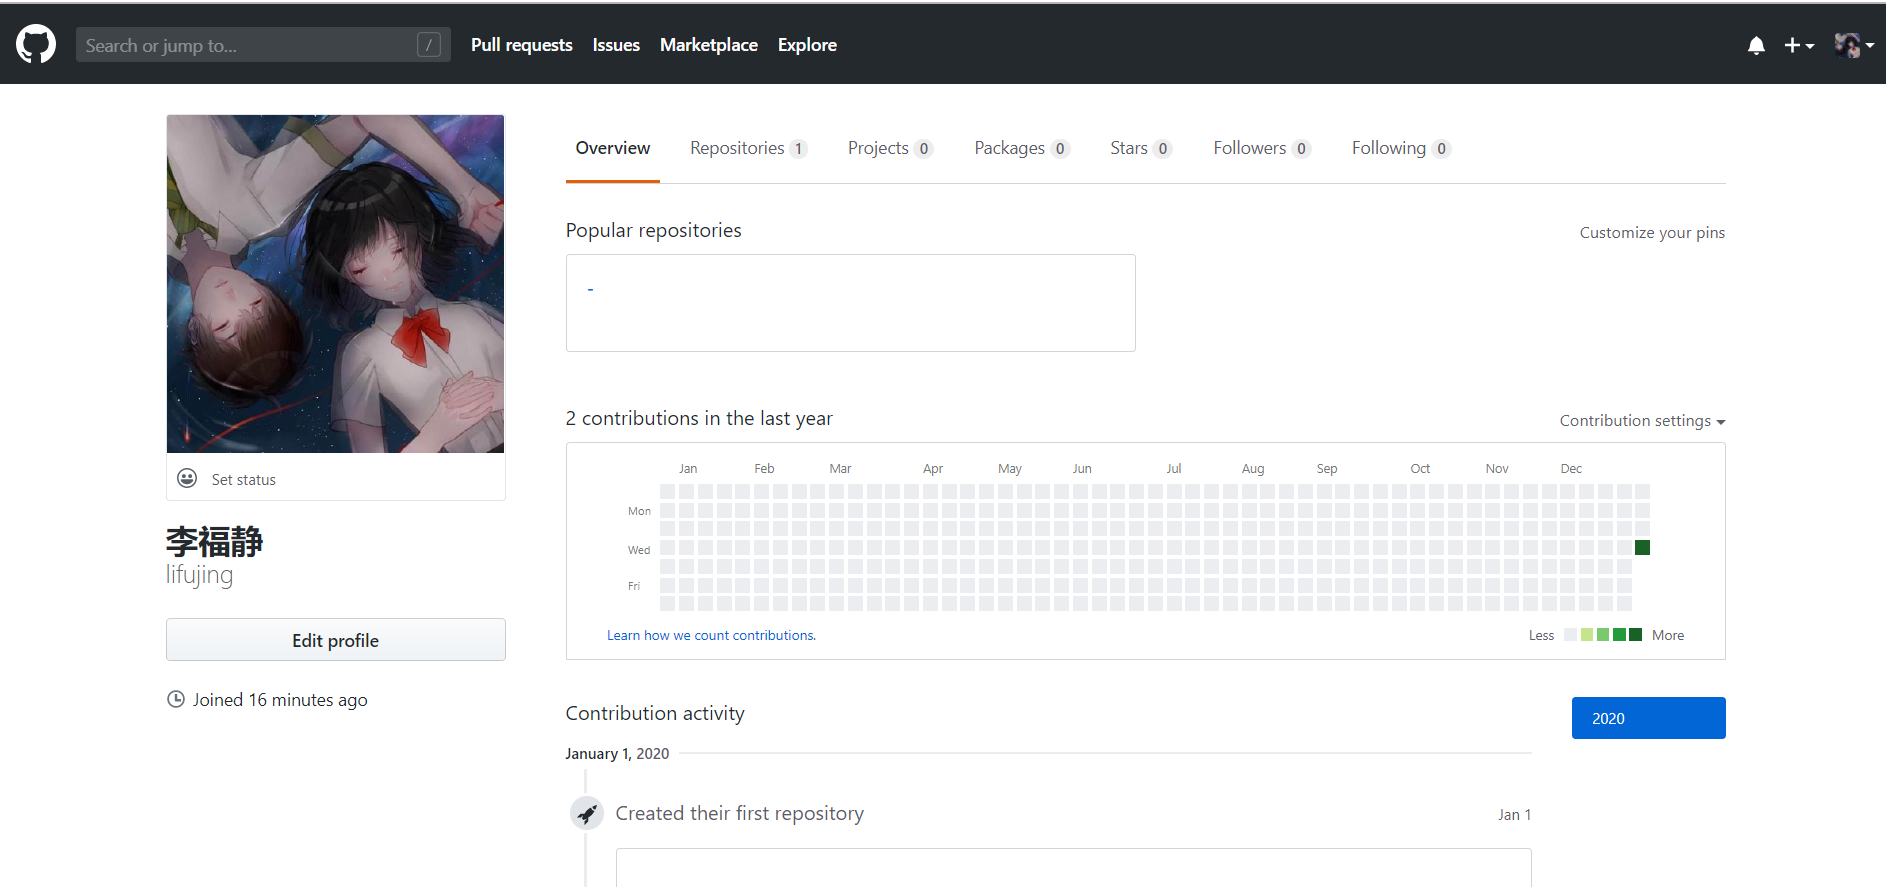
\includegraphics[scale=0.2]{x}
   	\caption{}
   	\label{fig:x}
   \end{figure}

   \item 观察者\par
   \begin{figure}[h!]
   	\centering
   	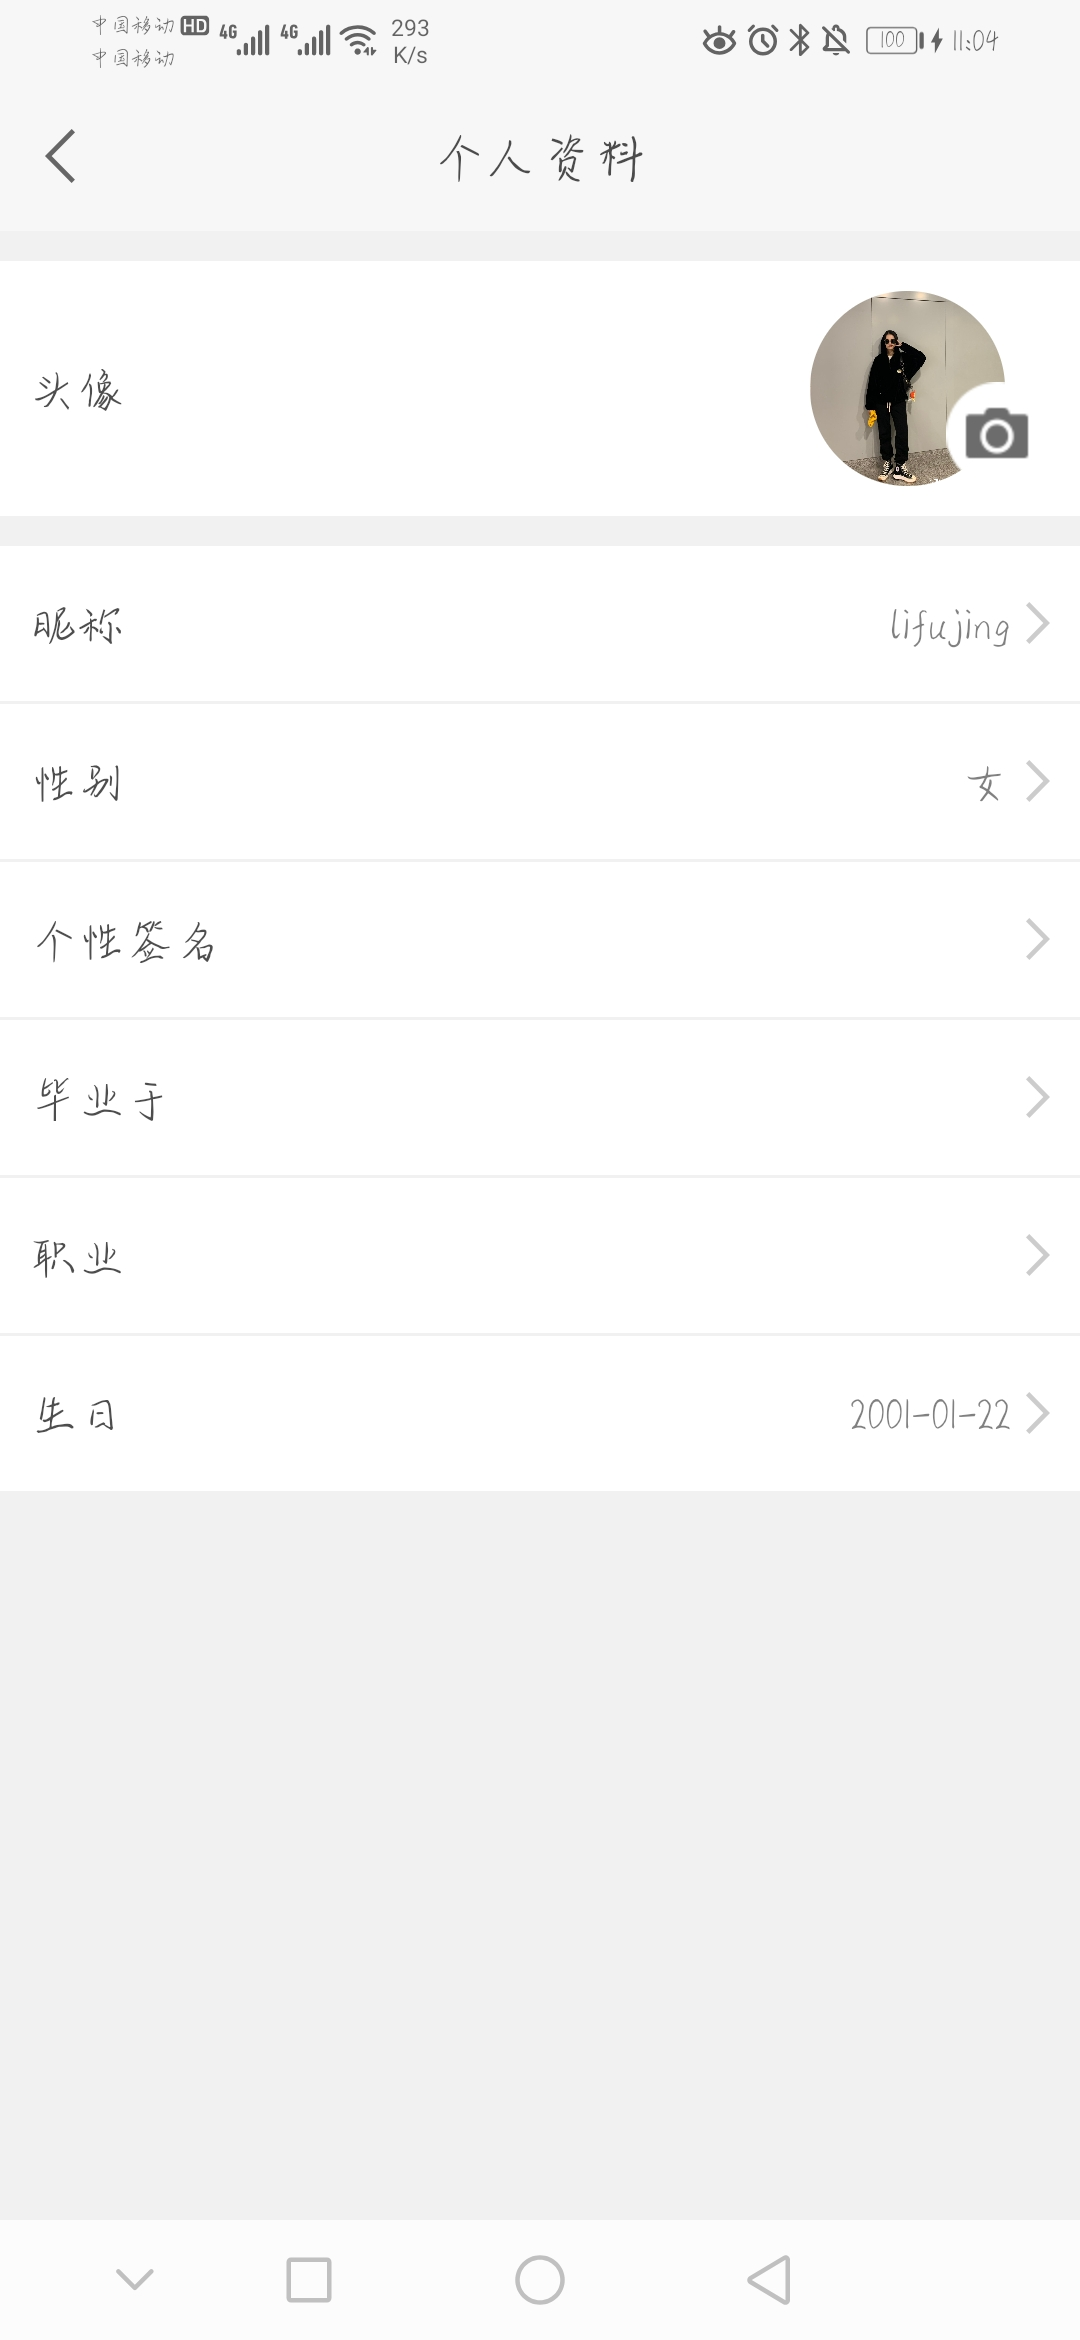
\includegraphics[scale=0.1]{b}
   	\caption{}
   	\label{fig:b}
   \end{figure}
   \newpage
   \item 学习强国\par
   \begin{figure}[h!]
   	\centering
   	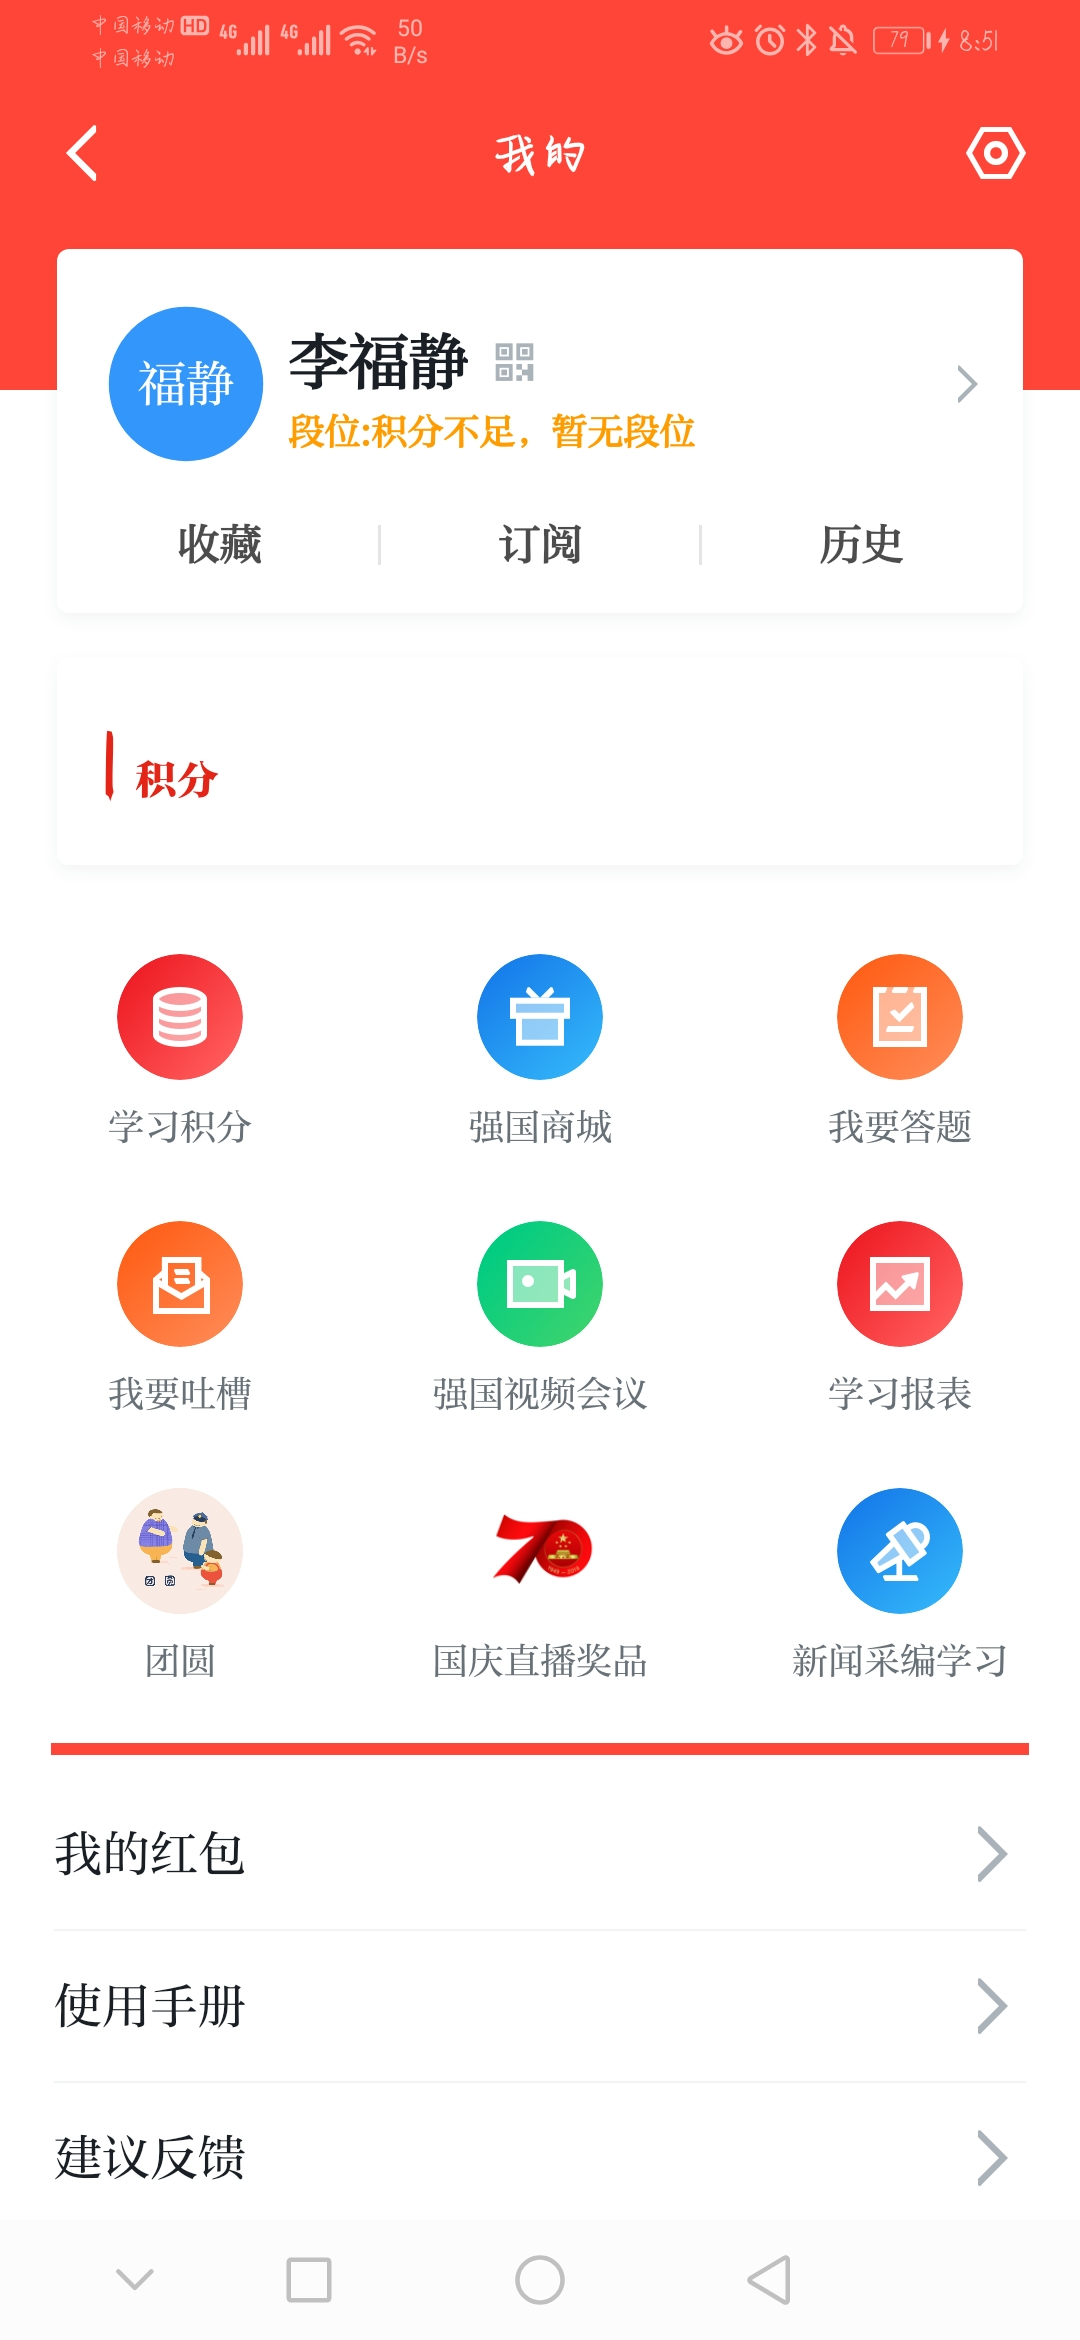
\includegraphics[scale=0.1]{c}
   	\caption{}
   	\label{fig:c}
   \end{figure}
   
  
   \item 哔哩哔哩APP\par
    \begin{figure}[h!]
    	\centering
    	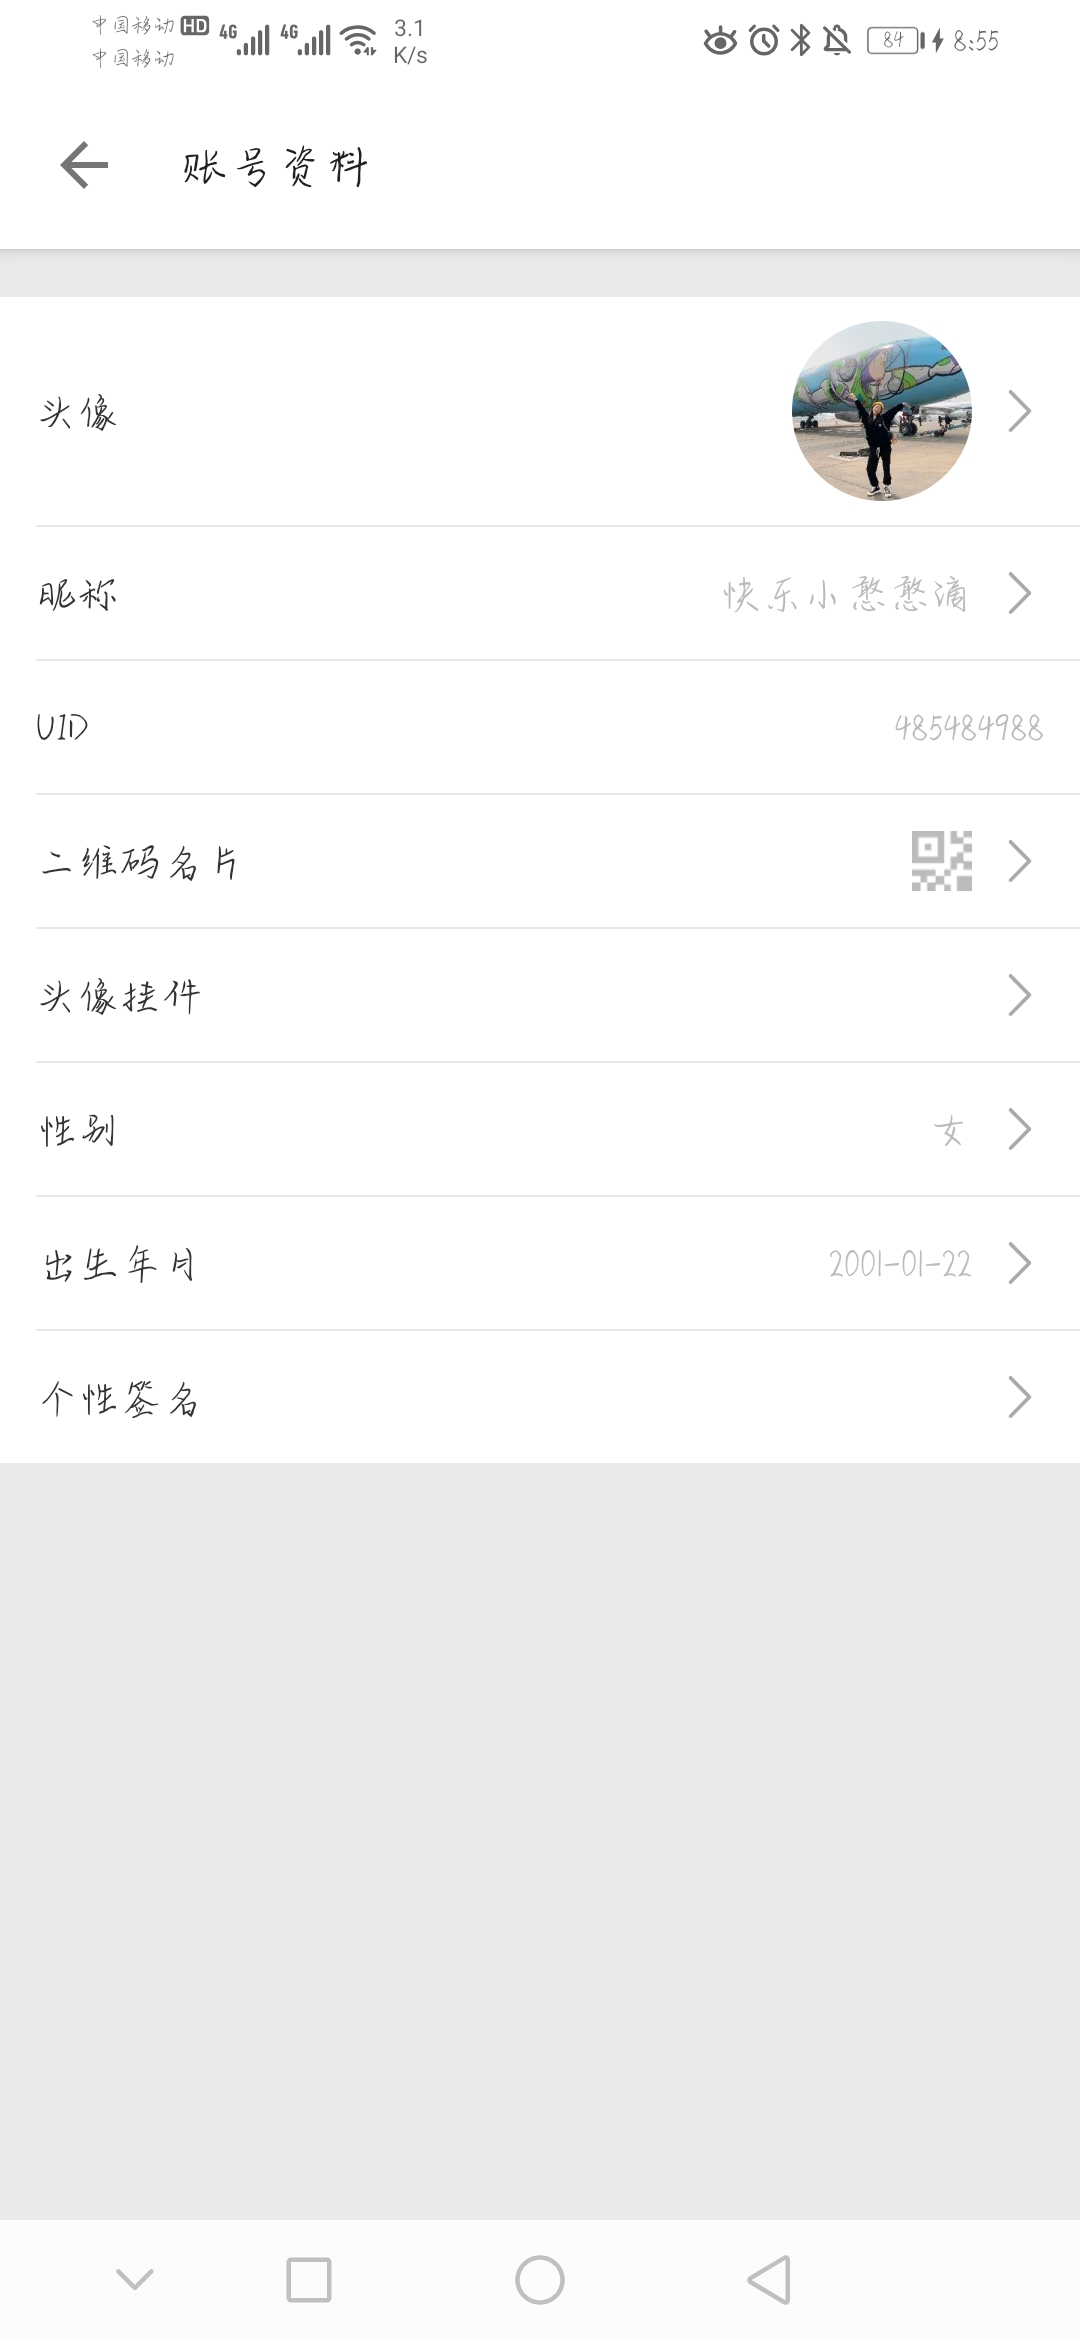
\includegraphics[scale=0.1]{a}
    	\caption{}
    	\label{fig:a}
    \end{figure}
    
    
    \newpage
    \item CSDN 个人网站截图:\par
    \begin{figure}[h!]
    	\centering
    	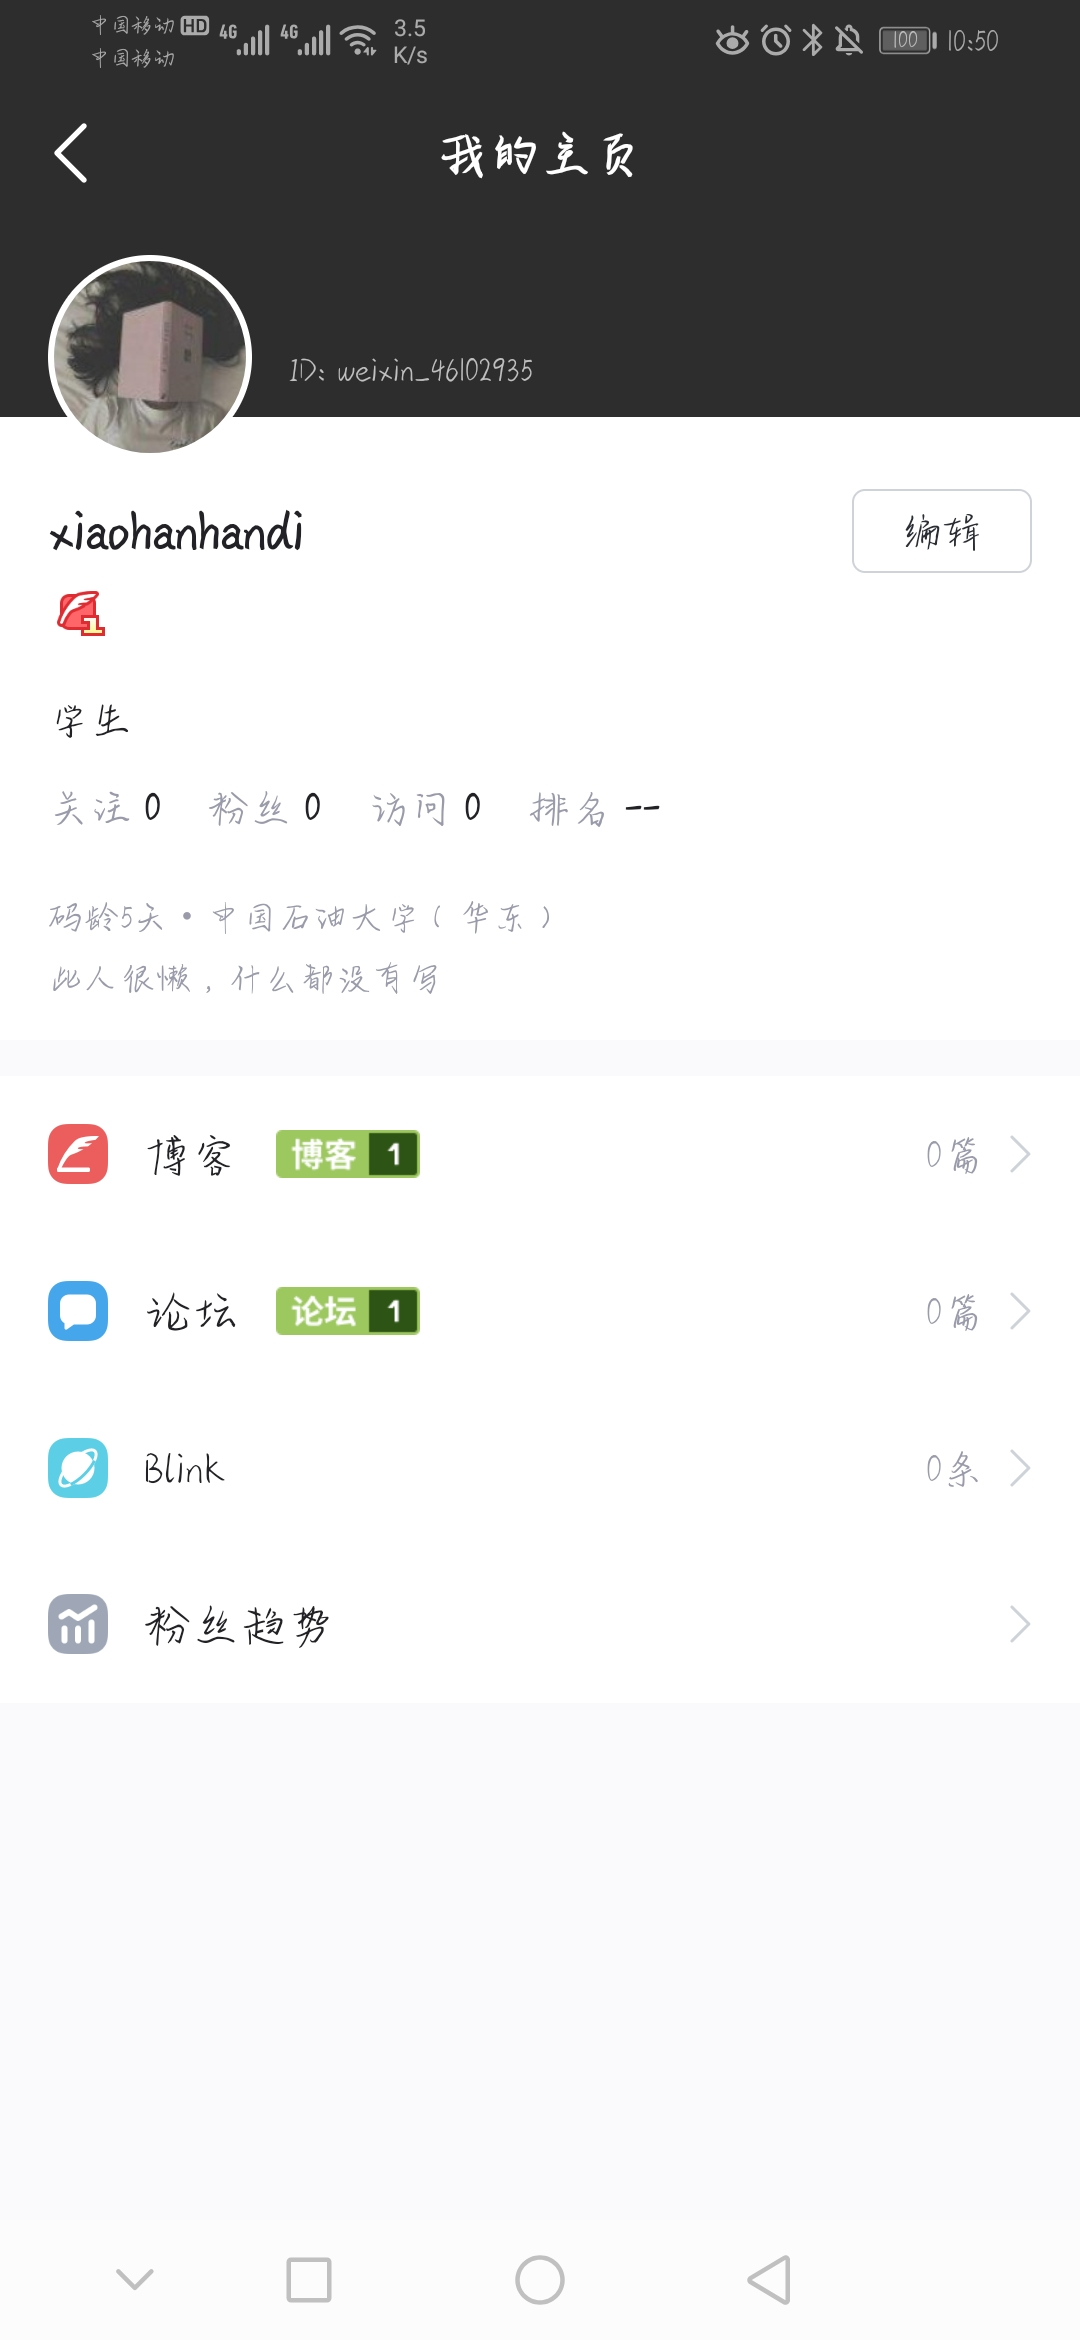
\includegraphics[scale=0.1]{s}
    	\caption{}
    	\label{fig:y}
    \end{figure}
    
   \item 博客园 个人网站截图:\par
   \begin{figure}[h!]
   	\centering
   	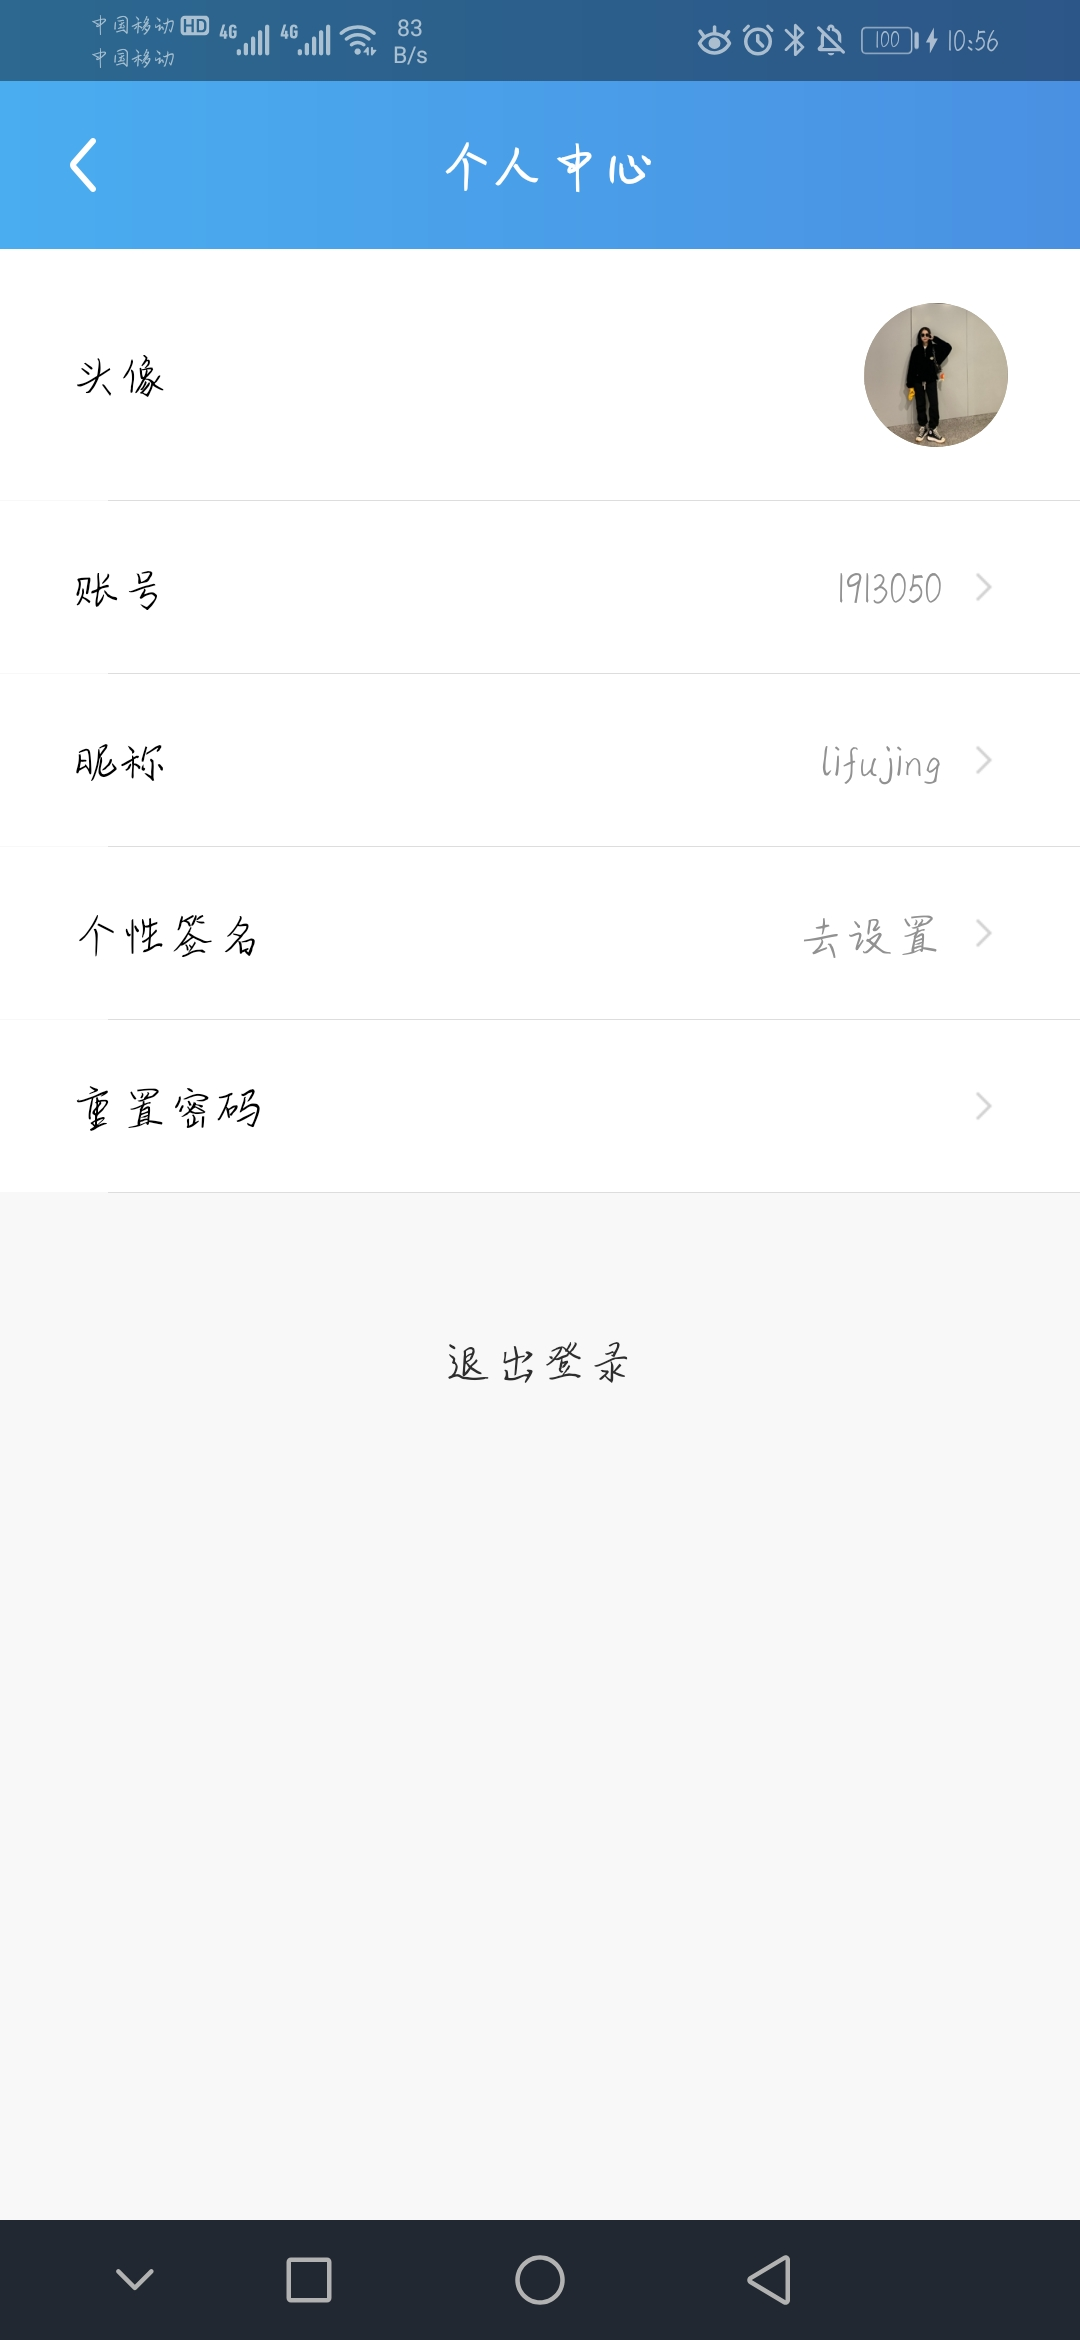
\includegraphics[scale=0.1]{k}
   	\caption{}
   	\label{fig:k}
   \end{figure}
   \newpage
    \item 小木虫 个人网址:http://muchong.com/bbs/space.php?uid=20345533\par
   个人网站截图:\par
   \begin{figure}[h!]
   	\centering
   	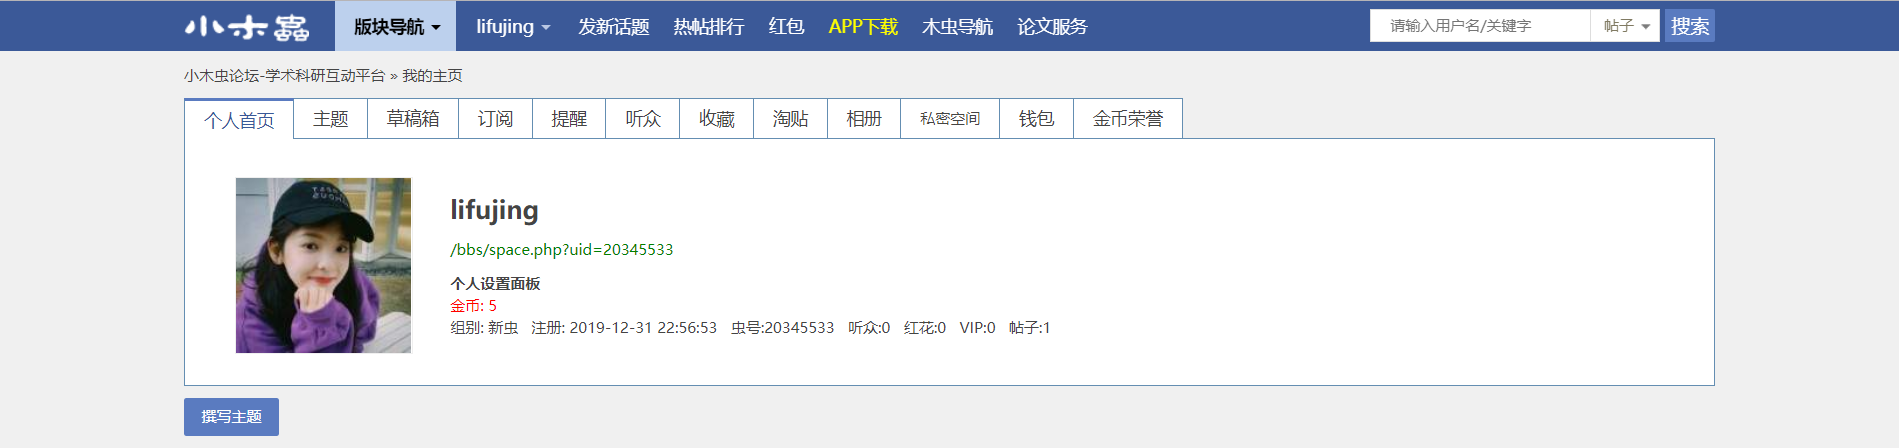
\includegraphics[scale=0.2]{mc}
   	\caption{}
   	\label{fig:mc}
   \end{figure}
   
\end{itemize}

















\hspace*{\fill} \\

\newpage
{\Large{\Large  参考文献:}}\par
[1] 朱坤,李金铭,张敬华.Relief算法最佳数学降维过程的程序实现[J].福建电脑,2012,28(01):141-142+128.\par
[2] 罗虹.计算机网络技术在通信工程项目管理中的应用初探[J].中外企业家,2019(36):66.\par
[3] 李立.计算机网络通信安全中数据加密技术的应用[J].计算机产品与流通,2019(11):32.\par
[4] Engineering - Computer Engineering; New Computer Engineering Findings from School of Computer and Communication Sciences Described (Analog Neural Networks with Deep-submicron Nonlinear Synapses)[J]. Computers, Networks , Communications,2019. \par
[5] 成晋军,张晓娟.云桌面VDI和VOI工作模式的协同研究[J].现代计算机,2019(31):38-41.\par
[6] 邓丽萍.基于Spice协议分块图像缓存优化设计与分析[J].福建教育学院学报,2019,20(04):120-125.\par
[7].杨振锋.云桌面技术及安全问题[J].信息与电脑(理论版),2018(05):26-27+30.\par
[8]. Yang Sheng. Design and Application of Desktop Cloud Experimental Teaching Platform[P]. Proceedings of the 2019 5th International Conference on Social Science and Higher Education (ICSSHE 2019),2019.\par

\end{document}
